%\documentclass[border={0.1cm 0.1cm 0.1cm 0.1cm}]{standalone}  %E,S,W,N
\documentclass{scrartcl}

\usepackage{amssymb}
\usepackage{amsmath}
\usepackage{graphicx}
\usepackage{tikz}
\usetikzlibrary{shapes} %for node shapes
\usetikzlibrary{calc}	%for centerarc

\begin{document}
	
	\hspace{-1cm}%		QWERTY
	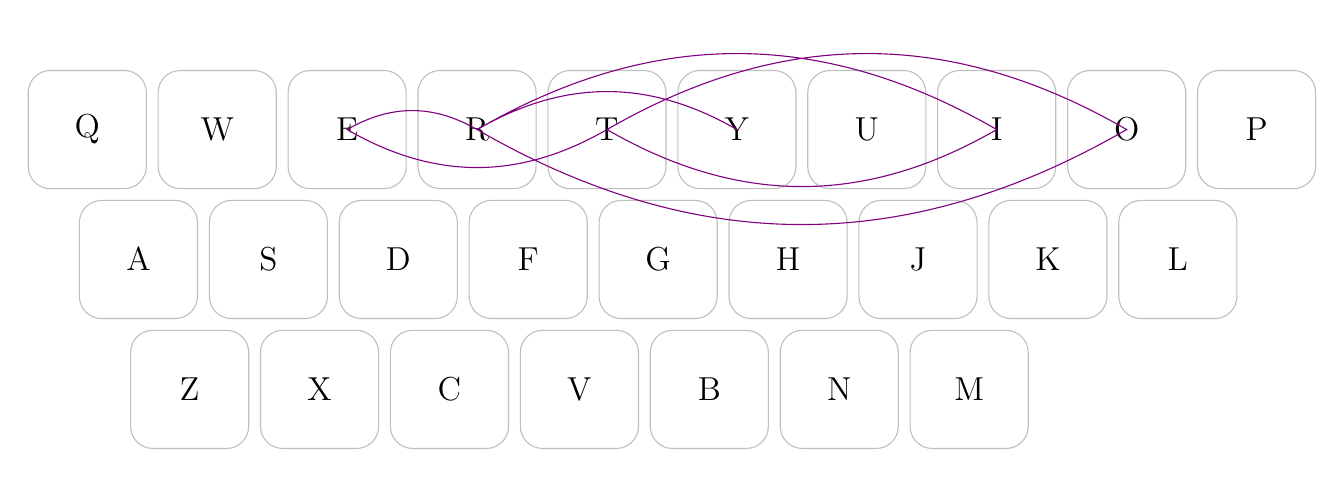
\begin{tikzpicture}	
	\def\s{0.75} %side length for keys
	\def\d{0.15} %distance between keys
	\foreach \i [count=\j] in {Q,W,E,R,T,Y,U,I,O,P}{ 
	\draw[rounded corners=8pt,gray!50!white] ({(2*\s+\d)*\j-\s},-\s) rectangle ++(2*\s,2*\s);
	\coordinate (\i) at ({(2*\s+\d)*\j},0);
	\node at (\i) {\large\i};
	}
	\foreach \i [count=\j] in {A,S,D,F,G,H,J,K,L}{ 
		\draw[rounded corners=8pt,gray!50!white] ({0.65+(2*\s+\d)*\j-\s},-3*\s-\d) rectangle ++(2*\s,2*\s);
		\coordinate (\i) at ({0.65+(2*\s+\d)*\j},-2*\s-\d);
		\node at (\i) {\large\i};
	}
	\foreach \i [count=\j] in {Z,X,C,V,B,N,M}{ 
		\draw[rounded corners=8pt,gray!50!white] ({1.3+(2*\s+\d)*\j-\s},-5*\s-2*\d) rectangle ++(2*\s,2*\s);
		\coordinate (\i) at ({1.3+(2*\s+\d)*\j},-4*\s-2*\d);
		\node at (\i) {\large\i};
	}
	
	%\draw[blue] (A)--(X)--(I)--(O)--(M)--(A)--(T)--(I)--(C)--(S);
	%\draw[blue] (A) to[bend left] (X) to[bend left] (I) to[bend left] (O) to[bend left] (M) to[bend left] (A) to[bend left] (T) to[bend left] (I) to[bend left] (C) to[bend left] (S);
	
	%\draw[green!60!black] (D)--(E)--(C)--(O)--(D)--(I)--(N)--(G);
	%\draw[green!60!black] (D) to[bend left] (E) to[bend left] (C) to[bend left] (O) to[bend left] (D) to[bend left] (I) to[bend left] (N) to[bend left] (G);
	
	%\draw[magenta] (C)--(O)--(D)--(E);
	%\draw[magenta] (C) to[bend left] (O) to[bend left] (D) to[bend left] (E);
	
	%\draw[red] (I)--(N)--(T)--(E)--(N)--(S)--(I)--(T)--(I)--(E)--(S);
	%\draw[red] (I) to[bend left] (N) to[bend left] (T) to[bend left] (E) to[bend left] (N) to[bend left] (S) to[bend left] (I) to[bend left] (T) to[bend left] (I) to[bend left] (E) to[bend left] (S);
	
	%\draw[yellow] (R)--(H)--(I)--(Z)--(O)--(M)--(E);
	%\draw[yellow] (R) to[bend left] (H) to[bend left] (I) to[bend left] (Z) to[bend left] (O) to[bend left] (M) to[bend left] (E);
	
	%\draw[violet] (T)--(E)--(R)--(R)--(I)--(T)--(O)--(R)--(Y);
	\draw[violet] (T) to[bend left] (E) to[bend left] (R) to[bend left] (R) to[bend left] (I) to[bend left] (T) to[bend left] (O) to[bend left] (R) to[bend left] (Y);
	\end{tikzpicture}
	
	
	\vspace{1.5cm}
	
	
	\hspace{-1cm}%		DVORAK
	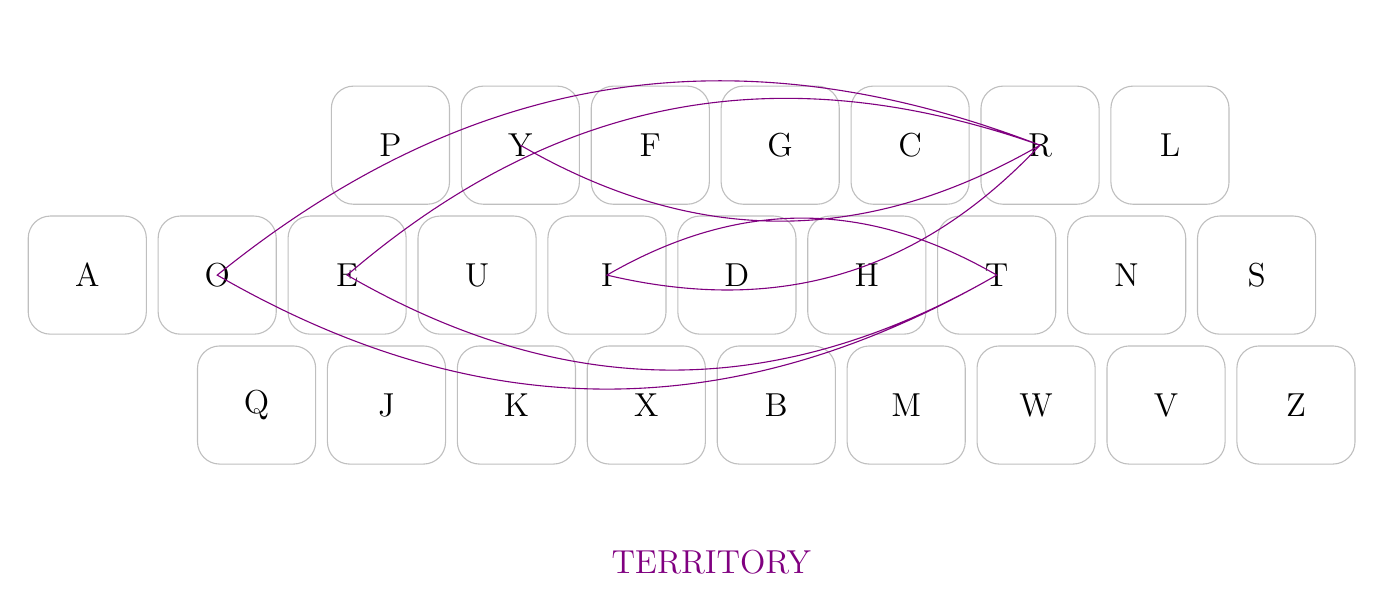
\begin{tikzpicture}	
	\def\s{0.75} %side length for keys
	\def\d{0.15} %distance between keys
	\foreach \i [count=\j] in {P,Y,F,G,C,R,L}{ 
		\draw[rounded corners=8pt,gray!50!white] ({6*\s+(2*\s+\d)*\j-\s},-\s) rectangle ++(2*\s,2*\s);
		\coordinate (\i) at ({6*\s+(2*\s+\d)*\j},0);
		\node at (\i) {\large\i};
	}
	\foreach \i [count=\j] in {A,O,E,U,I,D,H,T,N,S}{ 
		\draw[rounded corners=8pt,gray!50!white] ({0.65+(2*\s+\d)*\j-\s},-3*\s-\d) rectangle ++(2*\s,2*\s);
		\coordinate (\i) at ({0.65+(2*\s+\d)*\j},-2*\s-\d);
		\node at (\i) {\large\i};
	}
	\foreach \i [count=\j] in {Q,J,K,X,B,M,W,V,Z}{ 
		\draw[rounded corners=8pt,gray!50!white] ({2*\s+1.3+(2*\s+\d)*\j-\s},-5*\s-2*\d) rectangle ++(2*\s,2*\s);
		\coordinate (\i) at ({2*\s+1.3+(2*\s+\d)*\j},-4*\s-2*\d);
		\node at (\i) {\large\i};
	}

	%\draw[blue] (A)--(X)--(I)--(O)--(M)--(A)--(T)--(I)--(C)--(S);
	%\draw[blue] (A) to[bend left] (X) to[bend left] (I) to[bend left] (O) to[bend left] (M) to[bend left] (A) to[bend left] (T) to[bend left] (I) to[bend left] (C) to[bend left] (S);
	%\node[blue] at ({2*\s+1.3+(2*\s+\d)*4.5},-4*\s-2*\d-2) {\large AXIOMATICS};
	
	%\draw[green!60!black] (D)--(E)--(C)--(O)--(D)--(I)--(N)--(G);
	%\draw[green!60!black] (D) to[bend left] (E) to[bend left] (C) to[bend left] (O) to[bend left] (D) to[bend left] (I) to[bend left] (N) to[bend left] (G);
	%\node[green!60!black] at ({2*\s+1.3+(2*\s+\d)*4.5},-4*\s-2*\d-2) {\large DECODING};
	
	%\draw[magenta] (C)--(O)--(D)--(E);
	%\draw[magenta] (C) to[bend left] (O) to[bend left] (D) to[bend left] (E);
	%\node[magenta] at ({2*\s+1.3+(2*\s+\d)*4.5},-4*\s-2*\d-2) {\large CODE};
	
	%\draw[red] (I)--(N)--(T)--(E)--(N)--(S)--(I)--(T)--(I)--(E)--(S);
	%\draw[red] (I) to[bend left] (N) to[bend left] (T) to[bend left] (E) to[bend left] (N) to[bend left] (S) to[bend left] (I) to[bend left] (T) to[bend left] (I) to[bend left] (E) to[bend left] (S);
	%\node[red] at ({2*\s+1.3+(2*\s+\d)*4.5},-4*\s-2*\d-2) {\large INTENSITIES};
	
	%\draw[yellow] (R)--(H)--(I)--(Z)--(O)--(M)--(E);
	%\draw[yellow] (R) to[bend left] (H) to[bend left] (I) to[bend left] (Z) to[bend left] (O) to[bend left] (M) to[bend left] (E);
	%\node[yellow] at ({2*\s+1.3+(2*\s+\d)*4.5},-4*\s-2*\d-2) {\large RHIZOME};
	
	%\draw[violet] (T)--(E)--(R)--(R)--(I)--(T)--(O)--(R)--(Y);
	\draw[violet] (T) to[bend left] (E) to[bend left] (R) to[bend left] (R) to[bend left] (I) to[bend left] (T) to[bend left] (O) to[bend left] (R) to[bend left] (Y);
	\node[violet] at ({2*\s+1.3+(2*\s+\d)*4.5},-4*\s-2*\d-2) {\large TERRITORY};
	\end{tikzpicture}
	
\end{document}